\chapter{保拓扑的网格近似算法的分析和改进}

在上一章中我们详细介绍了Manish Mandad等人提出的保拓扑的网格近似算法\cite{isotopic-appro},和以往的算法相比,该算法通过细化和简化两个阶段的处理,能够取得更优的网格简化结果。然而,在细化过程中,该算法并没有去考虑三角网格本身存在的各向异性(我们在下面介绍),使用各向同性的3D Delaunay三角化来构建四面体网格$\tau$,这就使得后期需要通过消边操作来恢复三角网格的这个特性。本章我们将对该问题做一个分析阐述,并提出我们的改进策略。

\section{问题分析}
不难发现,在模型上的有些位置上,沿着不同的方向,对顶点的加一个相同大小的扰动(移动),所带来的误差的各不相同。如图\ref{fig:cylinder-deform}中的圆柱,顶点沿着不同方向上的扰动所带来的误差是不同的——在沿着轴方向上的误差最小,沿着圆周的方向上误差最大。这也是本文中所提的原三角网格上的各向异性的直观理解。相反的,在有些位置上,沿着不同方向对顶点做一个相同大小的扰动,误差的变化相同,比如球的表面,这是本文中各向同性的直观理解。因为模型存在各向异性,在网格简化的大部分情况下,会出现一些相对细长的三角面片(如图\ref{fig:cylinder-res1}所示)。而在Manish Mandad等人提出的保拓扑的网格近似算法在初始化阶段——细化时,使用了3D Delaunay三角化,这虽然能使得四面体更接近于正四面体,得到质量较好的四面体网格$\tau$,但是也意味着需要通过后序的简化操作去合并一部分质量较好的三角形从而获得与原网格的各向异性相符的相对细长的三角面片,而且后序的简化操作也未必能够很好地作出符合原三角网格各向异性特征的选择。因此,在这里我们期望能够找到一种更优细化方法,一种能够利用原三角网格上各向异性的特征的细化方法,从而得到一个更优的初始化四面体网格$\tau$。这样做不仅能使得算法的初始化状态更加精简,减少后序简化的步骤,而且因为考虑到了网格的各向异性,在不同的方向使用不同的边长,能够更好地降低误差得到更优的结果(在相同误差下顶点数量更少)。

\section{考虑各向异性的三角化}
为了得到这个更优的细化结果,我们需要一种能够利用原网格上各向异性信息的三角化方法来替换原来的3D Delaunay三角化。然而想出一种鲁棒可靠且能够直接依据原三角网格的各向异性信息,来对顶点做3D三角化的方法十分困难。虽然在最近二十年内,提出了许多基于Delaunay三角化技术的各向异性网格生成技术,但我们找不到一种既鲁棒又能满足我们这种固定顶点的各向异性三角化的需求的方法。
而另一种相对简单的策略是,我们根据原网格上的各向异性信息,对原网格所在的空间做一个使其趋向于各向同性的变形(warping),在形变的空间上做3D Delaunay三角化,再将这个三角化对应到原空间,从而得到一个各向异性信息的3D三角化结果。如图\ref{fig:cylinder-deform},图\ref{fig:cigar-deform}所示,我们通过形变将长方体形变成接近正方体,将细长的圆柱形变成一个扁平的圆盘,在形变之后的空间上做3D Delaunay三角化,映射到原空间,得到了带有各向异性信息的3D三角化结果。我们知道可以用黎曼度量(Riemannian metric)来表示网格上的各向异性或各向同性信息,因此,我们可以构造这样的黎曼度量,并利用它来指导我们形变。在2-manifold下的黎曼度量是一个对称正定的张量场$g$,通过它定义了两个切向量$u_1, u_2$的内积——$u_1^T g u_2$,从而对于任意非0向量$u$满足$u^T g u>0$。在这里,我们参考Daniele Panozzo等人提出的基于标架场(Frane Field)的形变算法\cite{frame-field-warping},根据网格上的黎曼度量信息,在网格上构建一个度量场,在这个度量场的指导下对网格进行变形使得最后的网格趋向于各向同性。然后依据网格的形变去计算出误差空间$\Omega$的形变$\Omega_d$使得网格趋向于各向同性,并在这个形变之后的误差空间$\Omega_d$上做3D Delaunay三角化。

\subsection{各向异性到各向同性的形变}
然而,要鲁棒地构建一个满足我们需求能够体现原网格上的各向异性信息的黎曼度量,既是一件十分具有挑战的事情,也是一件十分影响形变效果的事情。幸运的是,江腾飞等人提出了一种定义的黎曼度量的方法\cite{frame-field-gen}。当我们在三角网格上定义了这个张量场$g$之后,就可以根据这个度量场对模型做一个形变使得其趋向于各向同性。为了黎曼度量能充分体现原网格上的各向异性信息,在定制这个张量场$g$时,我们使用江腾飞等人提到的Directional length constraint\cite{frame-field-gen}——对于一个曲面$S_d$其Directional length constraint $(t, d, l) \in S_d$,表示在三角面片t上一个基向量在方向上的单位向量$d$满足$d^T g d = \frac{1}{l^2}$。参照Alliez等人的研究\cite{remesh-length},依据给定的Hausdorff误差范围$\varepsilon$,和某个方向上的曲率$\kappa$,在方向d上的局部长度(local size) $l$定义为:
\begin{equation}
  l = 2 \sqrt{\varepsilon(2/|\kappa| - \varepsilon)}
\end{equation}
从$l$的定义中不难看出,其很好地体现了我们所说的三角网格上的各向异性。在我们的算法中,我们添加主曲率方向上的两个Directional length constraint:
\begin{equation}
  d_1^T g d_1 = \frac{1}{l_1^2}, \quad  d_2^T g d_2 = \frac{1}{l_2^2}, \quad d_1^T g d_2 = 0
  \label{eq:calc_matric}
\end{equation}
在此约束基础上,再加上江腾飞等人提到的保证度量场光滑的约束,并进行优化计算,我们就得到了一高质量的能够体现原网格上各向异性信息的度量场。\par
在得到一个能够充分体现原网格上的各向异性信息的度量场后,参照Daniele Panozzo等人提出方法\cite{frame-field-warping},我们通过优化度量场上的一个能量,将原度量场变为尽可能各向同性的度量场,从而使得网格形变成为一个各向同性的网格。在我们离散的三角网格上,我们可以在每一个三角面片定义一个黎曼度量,从而在每一个三角面片t上,我们都可以根据\eqref{eq:calc_matric}计算出一个黎曼度量$g_t$,很容易发现我们在三角面片t上的一个理想的形变是$sQ\sqrt{g_t}$,这里s是一个自由变量表示放缩,Q是一个自由的旋转矩阵,这样就可以使得形变后的三角面片的local size在各个方向上都相等。然而现实中很难将所有的三角面片全部变形到最理想的状态,参照Daiele Panozzo等人的方法\cite{frame-field-warping},并根据我们的需求——需要使得主曲率方向上的local size尽可能一致,做一个修改,我们通过优化如下能量来计算每个三角面片t上的形变雅克比$J_t$:
\begin{equation}
  \epsilon(p') = \sum_{t\in S} \underset{Q \in SO(3)}{\text{min}} A_t \lVert J_t - sQ_t \widetilde{\sqrt{g_t}} \rVert_F^2
\end{equation}
这里,$Q_t$是一个3D空间中的旋转矩阵,其满足$Q_t^{-1} = Q_t^T$, $|Q_t| = 1$,$\widetilde{\sqrt{g}}_t$是矩阵$\sqrt{g_t}$的一个$3 \times 3$版本,而s则是我们为了增大解空间而加的一个放缩的自由变量——因为我们允许度量场两个方向(主曲率方向)上的相同比例的放缩,我们只期望其比例接近于1:1。在优化得到每个三角面片t上的形变雅克比$J_t$之后,我们就可以用它来计算形变之后的网格的每个顶点的新的坐标,从而我们就得到了一个趋于各向同性的网格$M_d$(如图\ref{fig:cylinder-deform}和图\ref{fig:cigar-deform}所示)。

\subsection{改进的三角化方法}
通过上述方法,我们将一个原网格M做了一个形变,生成了一个接近各向同性的网格$M_d$。然而,这并不足以满足我们的需求——我们真正想要做形变的是整一个误差空间$\Omega$,而不是原网格M。然而,对于已知M和$M_d$,去计算$\Omega$形变之后的$\Omega_d$,使得在空间$\Omega_d$上通过上述一系列简化操作后,得到的满足误差约束条件$\forall s_d \in S_d, \varepsilon(s_d)<1$的简化的网格$MS_d$,对应到原误差空间$\Omega$上得到的网格MS也仍然能够满足误差约束条件,这是一件非常具有挑战的事情。要得到形变之后的误差空间$\Omega_d$,也即需要知道形变之后的网格$M_d$上任意一处的新的误差范围。在这里我们对两个3D上的两个简单的网格椭球和圆柱做一个分析,对于三个半轴对应于x,y,z的且比例分别为1:1:4椭球(如图\ref{fig:ellipsoid-deform-tol}),假设我们的算法非常完美,在z轴上压缩成为原来的1/4,从而得到了一个球。那么显然,对于原误差空间$\Omega$,我们也只需要将其在z轴上压缩成为原来的1/4。而对于圆柱(如图\ref{fig:cylinder-deform-tol}),也假设我们的形变算法也非常完美,只是将其沿着对称轴的方向做了一个压缩,我们也只需要对其误差空间在沿着轴的方向做一个压缩。从中我们可以推测:网格$M_d$上任意一点处的误差厚度和原网格M在形变时,在该点处的曲率变化和法向上的放缩有关。而这件事情的挑战也在就在于去寻找这样一个关系,使得在形变空间$\Omega_d$上的误差约束条件和原空间$\Omega$上的误差约束条件一致。由于寻找该关系的难度很大,在这里我们使用一个更简单的替代方法,即我们根据$M \to M_d$,生成一个不那么准确地$\Omega_d'$ (按照网格整体的放缩对误差厚度做一个缩放,然后在$M_d$上以该误差厚度构建该误差空间$\Omega_d'$),得到与原空间内外壳采样点一一对应的采样点集合$S_d′$,我们在$\Omega_d'$上做3D Delaunay三角化得到$\tau′$,对应原空间中得到$\tau$,在原空间中去判断$\tau$是否满足误差约束条件。通过这种方式,我们就避免了去寻找这样一个复杂的关系,而且在得到具有各向异性的细化结果的同时,保证满足误差约束条件。

\begin{figure}[H]
  \centering
  \begin{subfigure}[b]{0.8\textwidth}
    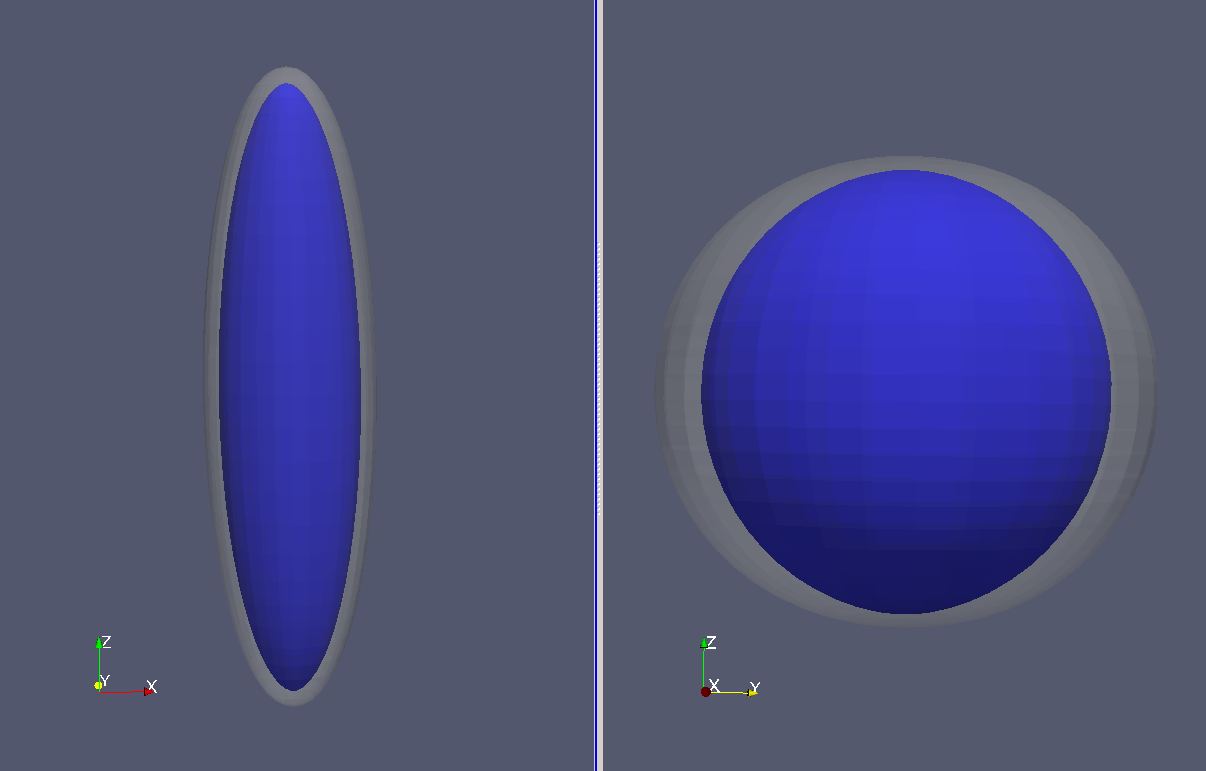
\includegraphics[width=\textwidth]{ellipsoid_deform_tolerance.png}
    \caption{当将椭球沿z轴压缩为原来的1/4之后,其误差空间的标准形变示意图。}
    \label{fig:ellipsoid-deform-tol}
  \end{subfigure}
  \begin{subfigure}[b]{0.8\textwidth}
      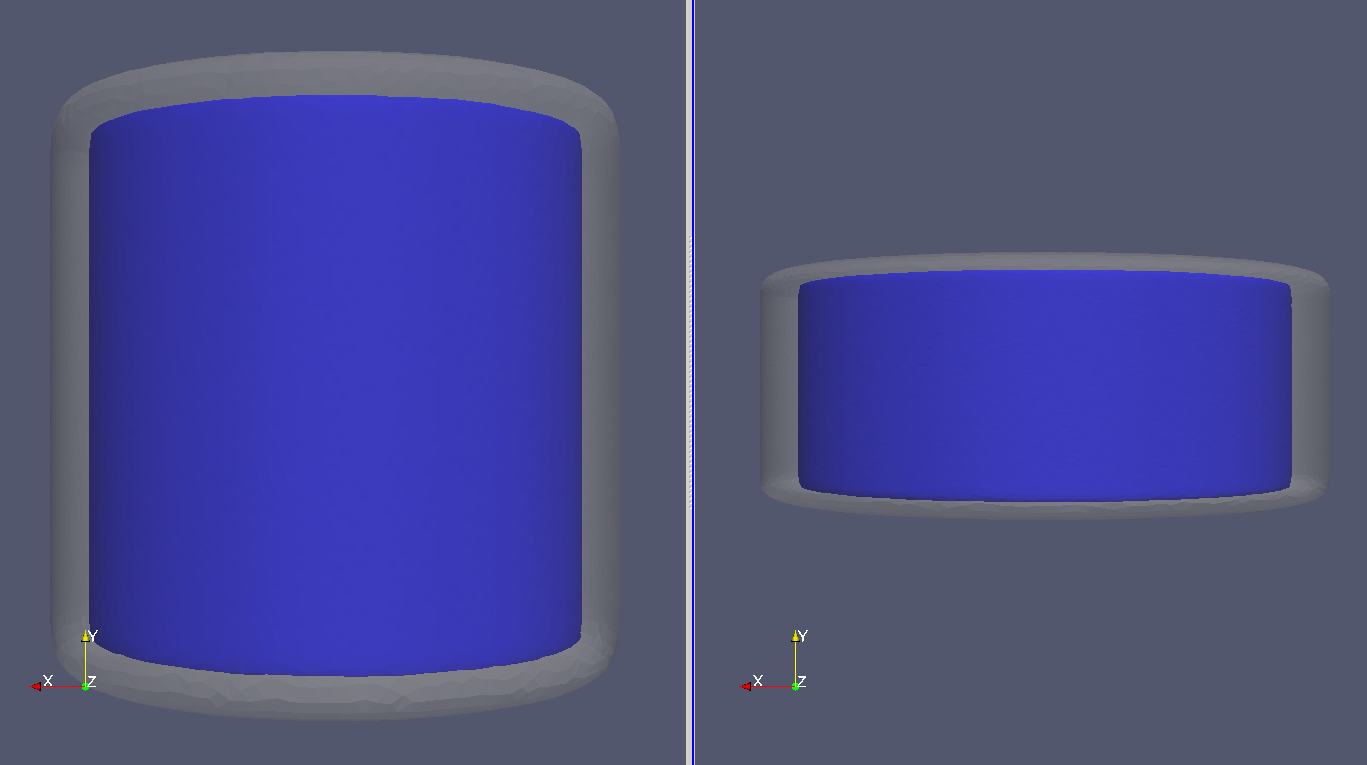
\includegraphics[width=\textwidth]{cylinder_deform_tolerance.png}
      \caption{当将圆柱沿对称轴压缩为原来的0.4倍之后,其误差空间的标准形变示意图。}
    \label{fig:cylinder-deform-tol}
  \end{subfigure}
  \caption[标准的误差空间形变示意图]{标准的误差空间形变示意图}
  \label{fig:deform-tol}
\end{figure}

\subsection{其他细节的修改}
当用带有各向异性的三角化方法替换原3D Delaunay三角化,并解决了除了误差约束条件的判断问题之后,我们还需要对采样点的选择策略,细化过程中对于无法满足法向约束条件的四面体的处理方法做一个修改。在细化算法中,通过贪心地选取误差最大的顶点加入$\tau$中,以期快速地使得误差约束条件得到满足。不难发现,一个采样顶点的加入,会使得其周围的采样顶点的误差迅速下降,而对离其较远的区域则无影响。因此,我们认为原算法的一个假设是最大误差采样点的周围会有较多的大误差采样点。而在我们现在的算法中,由于我们使用的带有各向异性的三角化方法是在$\Omega_d$的空间中做3D Delaunay三角化,而我们在$\Omega$和$\Omega_d$上的误差函数并不完全一致(上面我们提到想要找到一个与原误差空间$\Omega$的误差函数一致的形变误差空间$\Omega_d$非常困难),因此,我们这里有两种误差:原空间上的误差和形变空间上的误差。在我们的算法中我们同时维护这两个误差,以形变空间中的误差做为优先级排序的参照,并以原空间的误差是否超过误差边界作为采样点是否需要加入四面体网格τ的判断条件。也即每次从在原空间中超过误差边界的采样点中,选取在形变空间中误差最大的采样点加入到$\tau$中。实验证明,这种策略与选取在原空间中误差最大的采样点的策略相比能够得到更好的细化结果(顶点数量更少)。另外,对于不满足法向约束条件的四面体,由于现在的三角化方法,以原来的方法——在原空间中选取离其球心最近的采样点可能无法破坏该四面体。因此,我们选取在形变空间中离该四面体球心最近的采样点加入到$\tau$中。在得到一个考虑到原网格上各向异性信息的细化结果之后,剩下的简化处理我们与原算法一致,这里不再赘述。

\section{本章小结}
在本章,我们通过对原算法的分析,发现其第一步细化并没有考虑原网格上的各向异性信息,而用了3D Delaunay三角化来构建四面体网格$\tau$。这样虽然能够获得一个质量较好地四面体网格$\tau$,但与此同时,也意味着需要通过后序的简化操作去生恢复这样的各向异性信息,而且后序的简化操作也不一定能够很好地恢复(可能会由于边的Kernel Region小,空间采样点的稀疏等原因导致有些边无法合并)。因此,我们希望能够在细化阶段将原网格上的各向异性信息利用起来,得到一个更优的细化结果,从而减少后序简化操作的负担,并优化简化结果。然后我们介绍了我们的具体做法:我们首先通过参照江腾飞等人提出的自定义的黎曼度量的方法\cite{frame-field-gen},在原网格上构建了一个体现其各向异性信息的度量场,然后依据Daniele Panozzo等人提出的基于标架场的形变算法\cite{frame-field-warping},用该度量场构建并优化一个能量,从而将带有各向异性信息的原网格M形变成为一个趋于各向同性的网格$M_d$。然后根据$M \to M_d$,在$M_d$上构建一个形变后的误差空间$\Omega_d$。通过在形变的误差空间$\Omega_d$上的3D Delaunay三角化来得到在原空间考虑到原网格上各向异性信息的三角化,从而达到了我们期望,优化了细化结果。
